\documentclass[a4paper,11pt,oneside]{article}

\author{ J.R. Leeman} 
\title{Python Biax Data Reader: biaxread}

\usepackage{amsmath}
\usepackage{graphicx}
\usepackage{setspace}
\usepackage{indentfirst}
\usepackage{fullpage}
\usepackage{epstopdf}
\usepackage{listings}
\usepackage{color}
\usepackage{caption}

\definecolor{dkgreen}{rgb}{0,0.6,0}
\definecolor{gray}{rgb}{0.5,0.5,0.5}
\definecolor{mauve}{rgb}{0.58,0,0.82}

\lstset{frame=tb,
  language=Python,
  aboveskip=3mm,
  belowskip=3mm,
  showstringspaces=false,
  columns=flexible,
  basicstyle={\small\ttfamily},
  numbers=left,
  numberstyle=\tiny\color{gray},
  keywordstyle=\color{blue},
  commentstyle=\color{dkgreen},
  stringstyle=\color{mauve},
  breaklines=true,
  breakatwhitespace=true
  tabsize=3
}


\begin{document}
\maketitle
\newpage

\section{Purpose}
This script was designed to read data into an easy to use format from the text output of xlook.  Data is read, the header parsed for column names, lengths, etc., and a rec array returned that is easy to access and call from within a script.  Column names are used to call the data columns, so as long as consistent naming is used the column order in the file is irrelevant.

\section{Description}

biaxread first opens the text file with a standard open command.  We know that each column in the data is written as 12 characters wide.  The first line of the header is the number of records, the second is the column number, the third the column headings, the fourth the column units, and the fifth the number of records in each column.  This information if parsed and stored.  A rec array is created with the numpy package and the labels set of the column names that were parsed.  Finally the array is populated with data and the final product returned to the calling script.

A new set of improvements would be to add a cutting tool or a way to interface the script with the Pandas data handling library.

\section{Cautions}
A few cautions should be observed when using the biaxread script:

\begin{enumerate}
\item The empty array is shaped by row number information from the header.  If a datafile is cut, but the header is left unmodified there will be many extra zero data pairs at the end of the array.
\end{enumerate}

\section{Usage}

First process the experimental data in xlook and output a text file with headers.  To do this input \emph{type 0 -1 1 12 p4074\_data.txt} at the xlook command line or add it to the data reduction file.  Be sure to correct any column or row number specifications here.  Start IPython or open your own python script.  Import biax read and pass the function ReadBiax the name of the text output file from xlook.  The array is now returned and ready to use.  

\section{Acknowledgements}
Thank you to Marco Scuderi for using the code and being patient as little issues were worked out.  This code is free for all to use with proper acknowledgement.  Please send any bug reports to kd5wxb@gmail.com.

\noindent%
\begin{minipage}{\linewidth}
\makebox[\linewidth]{%
      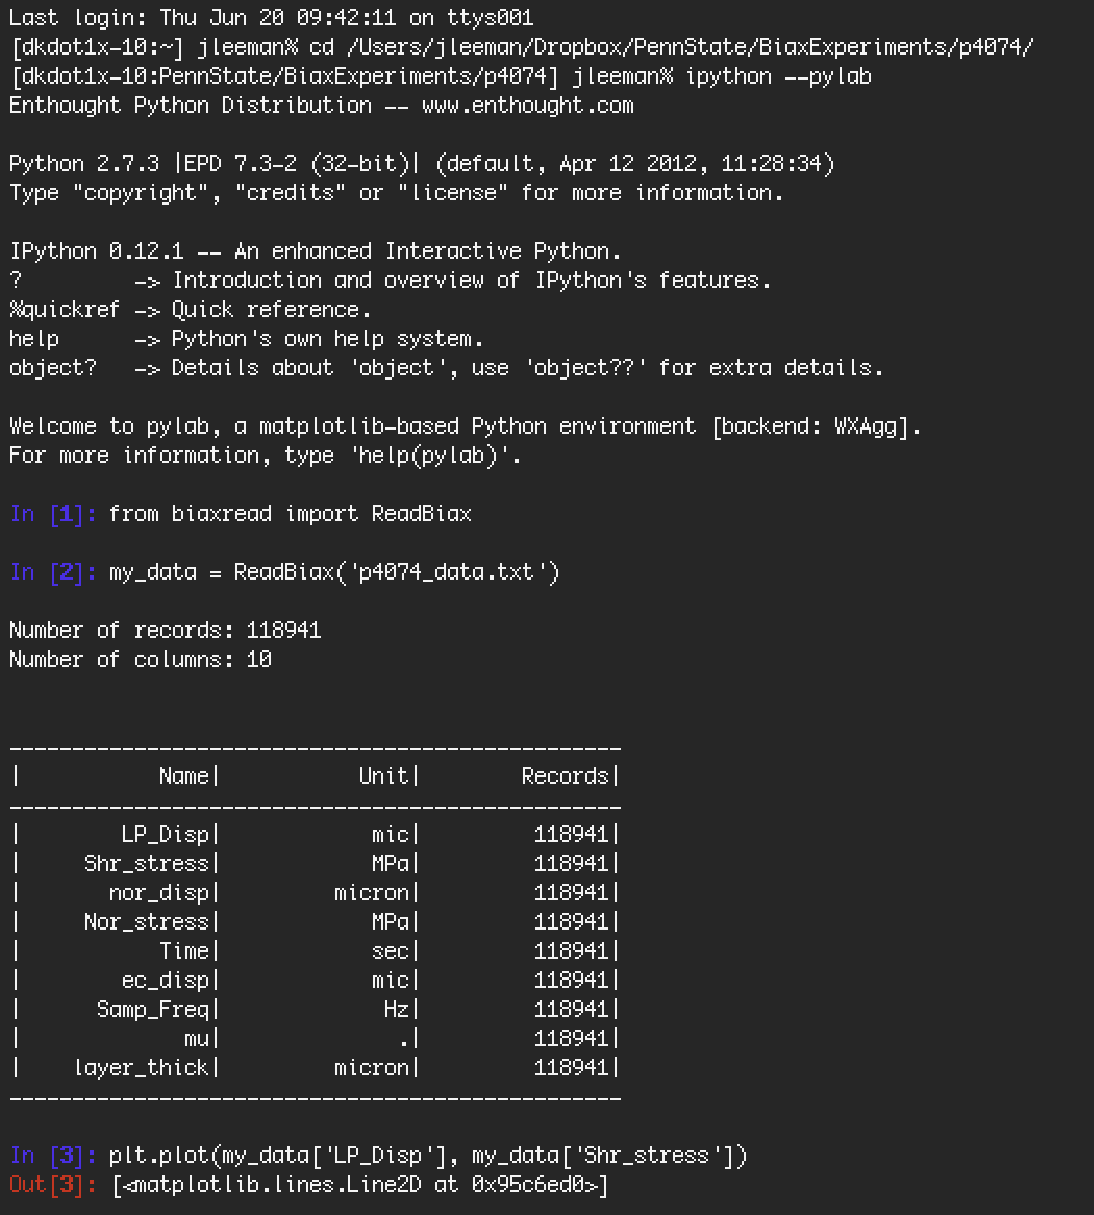
\includegraphics[scale=0.7]{screenshot.pdf}}
\end{minipage}


\newpage

\section{Code}
\begin{lstlisting}
import numpy as np
import sys

def ReadBiax(f_name):
    """
    Takes a filename containing the text output (with headers) from xlook and
    reads the columns into a rec array for easy data processing and access.
    """

    filename = f_name

    datafile = open(filename,'r')
    
    col_width = 12 # Columns are 12 char wide in header
    
    # First line of the file is the number of records
    num_recs = datafile.readline()
    num_recs = int(num_recs.strip('number of records = '))
    print "\nNumber of records: %d" %num_recs
    
    # Second line is column numbers, we don't care so just count them
    num_cols = datafile.readline()
    num_cols = num_cols.split('col')
    num_cols = len(num_cols)
    print "Number of columns: %d" %num_cols
    
    # Third line is the column headings
    col_headings_str = datafile.readline()
    col_headings_str = col_headings_str[5:-1]
    col_headings = []
    for i in xrange(len(col_headings_str)/12):
        heading = col_headings_str[12*i:12*i+12].strip()
        col_headings.append(heading)

    # Fourth line is column units
    col_units_str = datafile.readline()
    col_units_str = col_units_str[5:-1]
    col_units=[]
    for i in xrange(len(col_units_str)/12):
        heading = col_units_str[12*i:12*i+12].strip()
        col_units.append(heading)
    col_units = [x for x in col_units if x != '\n']  #Remove newlines
    
    # Fifth line is number of records per column
    col_recs = datafile.readline()
    col_recs = col_recs.split('recs')
    col_recs = [int(x) for x in col_recs if x != '\n']
    
    # Show column units and headings
    print "\n\n-------------------------------------------------"
    print "|%15s|%15s|%15s|" %('Name','Unit','Records')
    print "-------------------------------------------------"
    for column in zip(col_headings,col_units,col_recs):
        print "|%15s|%15s|%15s|" %(column[0],column[1],column[2])
    print "-------------------------------------------------"
    
    # Read the data into a numpy recarray
    dtype=[]
    dtype.append(('row_num','float'))
    for name in col_headings:
        dtype.append((name,'float'))
    dtype = np.dtype(dtype)
    
    data = np.zeros([num_recs,num_cols])
    
    i=0
    for row in datafile:
        row_data = row.split()
        for j in xrange(num_cols):
            data[i,j] = row_data[j]
        i+=1
    data_rec = np.rec.array(data,dtype=dtype)
    
    datafile.close()
    
    return data_rec

\end{lstlisting}

\end{document}